\chapter{Large Language Models (LLMs)}
\pagestyle{fancy}\lhead{\textbf \footnotesize\it{Enhancing Legal Information Access with Retrieval Augmented LLMs for Juridical Data}}
\pagestyle{fancy}\chead{} \pagestyle{fancy}\rhead{}
\pagestyle{fancy}\lfoot{\textbf {\small\it{Univ-Mascara/Computer Science: 2025}}} 
\pagestyle{fancy}\cfoot{} \pagestyle{fancy}\rfoot{\thepage}
%%%%%%%%%%%%%%%%%%%%%%%%%%%%%%%%%%%%%%%%
\section{Introduction} \label{start1}
Large Language Models (LLMs) represent a transformative leap in Natural Language Processing (NLP), allowing machines to perform complex language tasks with remarkable accuracy. From generating coherent text to answering nuanced questions, LLMs have pushed the boundaries of what AI can achieve. This chapter delves into the architecture and principles behind LLMs, their development through scaling and training techniques, and the models that have defined this field. It also addresses the challenges these models face and their expanding role in various real-world applications. 

\section{Natural language processing (NLP)}
Natural Language Processing (NLP) is a field within artificial intelligence (AI) that concentrates on the interaction between computers and human language. It involves the development of algorithms and models  that allow machines to comprehend, interpret, and generate human language in a meaningful context.NLP is crucial for enabling computers to process and respond to human language effectively, as demonstrated by features like Google's predictive text in keyboards and language translation systems that manage multiple languages efficiently \cite{murugan2024nlp}

\subsection{Historical development of NLP}
The figure below presents a timeline outlining the key developments in Natural Language Processing (NLP)  beginning with rule-based approaches in the 1950s and progressing through the rise of statistical methods and early neural networks in the late 1980s. It then highlights the impact of deep learning from the 2000s onward, leading to the development of pre-trained models like BERT and GPT. The timeline concludes with the emergence of large language models (LLMs) from 2019 to the present, marking a significant shift in NLP research and applications.
\begin{figure}[htbp]
	\centerline{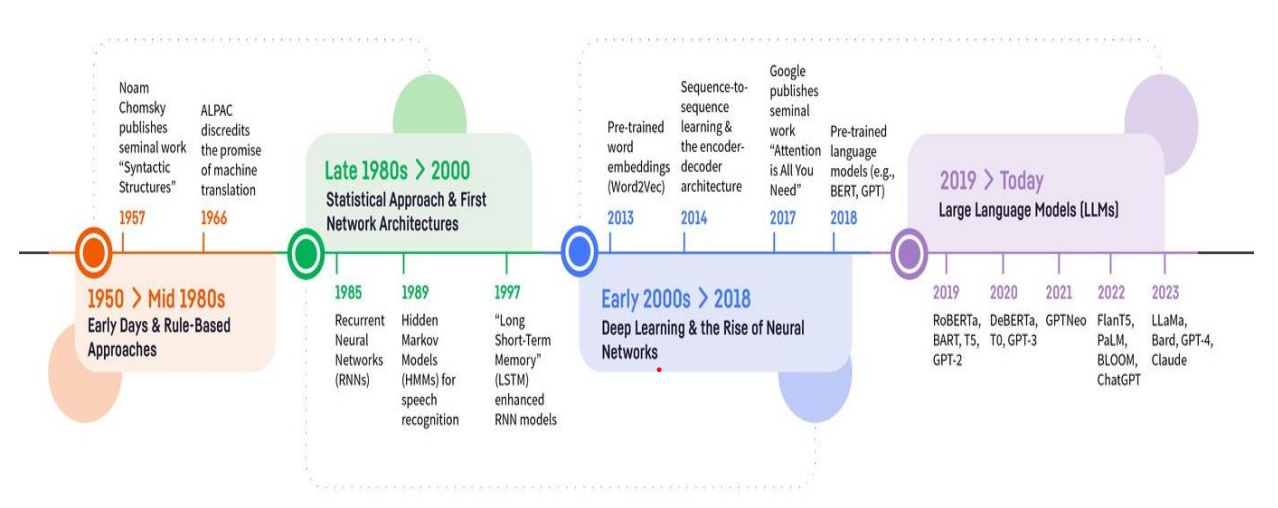
\includegraphics[scale=.7]{Figures/the_historyOf_nlp.png}}
	\caption{The Vauquois triangle, illustrating the foundations of machine translation.}
	\label{the_historyOf_nlp.png}
\end{figure}

\subsection{Importance of natural language processing}

\begin{enumerate}
	\item \textbf{Efficient Data Processing:} NLP enables businesses to process and analyze large volumes of unstructured, text-heavy data that would be challenging to handle otherwise..

	\item \textbf{Understanding Human Language:}NLP can interpret complex language elements, such as acronyms, abbreviations, and context, improving the accuracy of machine learning models..
	
	\item \textbf{Advancements in Technology:}Improvements in deep learning and machine learning have made NLP more effective, expanding the types of data that can be analyzed.
	
	\item \textbf{Natural Interactions:} NLP allows users to interact naturally with AI chatbots and voice assistants, like Siri, without needing to use specific,predefined\cite{techtarget_nlp}.
	
\end{enumerate}

\section{Neural Networks in NLP}
A neural network, or artificial neural network, is a machine learning algorithm inspired by the human brain. It is a key component of deep learning, a branch of machine learning effective in solving complex problems like image recognition and language processing. Unlike traditional computer programs that use a step-by-step algorithmic approach, neural networks learn from examples, mimicking the way neurons in the human brain operate. They consist of interconnected nodes (processing elements) that work together in parallel to solve specific problems. \\
A neural network has three basic sections, or parts, each composed of "nodes." \\ The input layer is the first part, receiving raw data, with each node (or neuron) representing a feature of this data. The hidden layers, which form the intermediate section, perform various transformations and computations, enabling the network to learn complex patterns and relationships. Finally, the output layer, which is the last part, produces the network's output, with the number of nodes corresponding to the desired output classes or regression values \cite{murugan2024nlp}.
\begin{figure}[htbp]
	
	\centerline{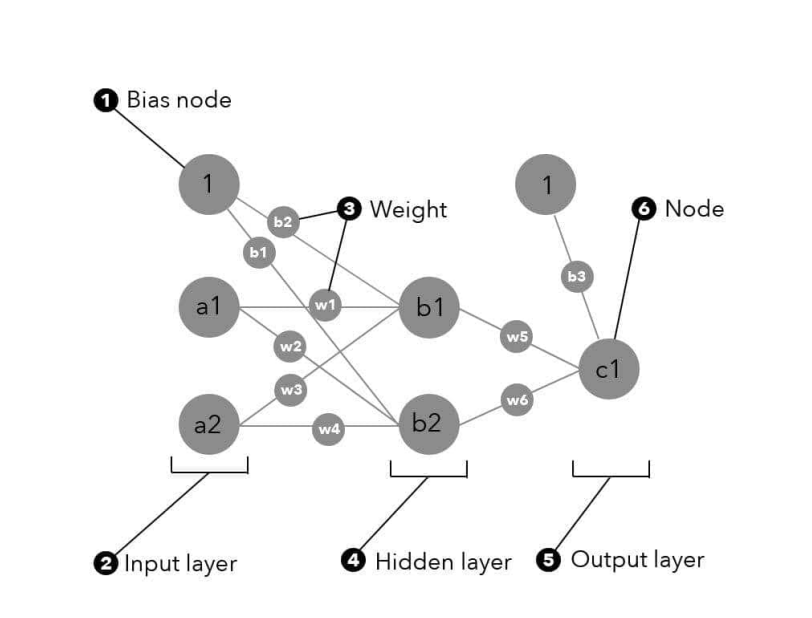
\includegraphics[width=.7\linewidth]{Figures/ANN.png}}
	\caption{Artificial Neural Network (ANN).}
	\label{ANN.png}
\end{figure}  

\subsection{Basics Concepts in Neural Networks}
\textbf{Weights} \\
Variables on the edges between nodes that are multiplied with node outputs to form the input for the next layer.Weights are crucial for training and tuning a neural network and are often initialized within a range of -1 to 1.  \\ \\ 
\textbf{Biases} \\
Additional nodes in hidden and output layers that connect to every node within their respective layers but not to the previous layer. Biases add a constant value (typically 1 or -1) to the input of a layer, helping shift the activation function and aiding in effective learning. 
\textbf{Activation Functions} \\
These functions introduce non-linearity to the network, enabling it to learn and model complex data patterns. Common activation functions include the sigmoid, hyperbolic tangent (tanh), and rectified linear unit (ReLU). \cite{taylor2017neural}.

\subsection{ Recurrent Neural Networks (RNNs)}
Recurrent neural networks (RNNs) are a type of neural network designed for processing sequential data, such as text or time series, by effectively handling variable-length inputs. An RNN consists of a hidden state h and an optical output y, which operate on a variable  sequence x=($x_1$....$x_t$)At each time step t, the hidden state $h^t$
of the RNN is updated according to the function $h^{(t)} = f(h^{(t-1)}, x_t)$
where f is a non-linear activation function, such as a logistic sigmoid or a more complex long short-term memory (LSTM) unit. This design allows RNNs to remember past inputs and incorporate them into future outputs, enabling them to recognize patterns that occur at multiple positions within a sequence. Additionally, RNNs utilize parameter sharing across time steps, which helps in generalizing across sequences of varying lengths and learning complex dependencies over time. Despite challenges with long-term dependencies, RNNs are particularly effective for tasks requiring context or sequential understanding, making them valuable for various applications, including time series analysis and natural language processing\cite{cho2014learning} 
\begin{figure}[htbp]
	
	\centerline{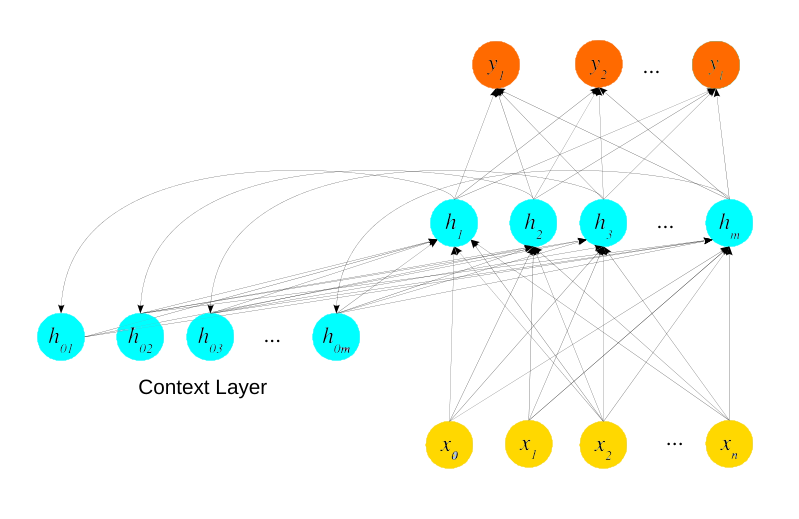
\includegraphics[width=1\linewidth]{Figures/RNN.png}}
	\caption{RNN Architecture.}
	\label{RNN.png}
\end{figure}
\subsection{ Long-Short Term Memory (LSTM)}
Long Short-Term Memory (LSTM) networks, designed by Hochreiter and Schmidhuber, are an improved version of recurrent neural networks (RNNs) designed to learn long-term dependencies in sequential data, making them suitable for tasks like time series forecasting and language translation
They address the limitations of traditional RNNs by introducing a memory cell that maintains information over extended periods. This memory cell is regulated by three gates—input, forget, and output gates—which control the flow of information in and out of the cell as shown in the fig \cite{geeksforgeeks_lstm}
\begin{figure}[htbp]
	\centering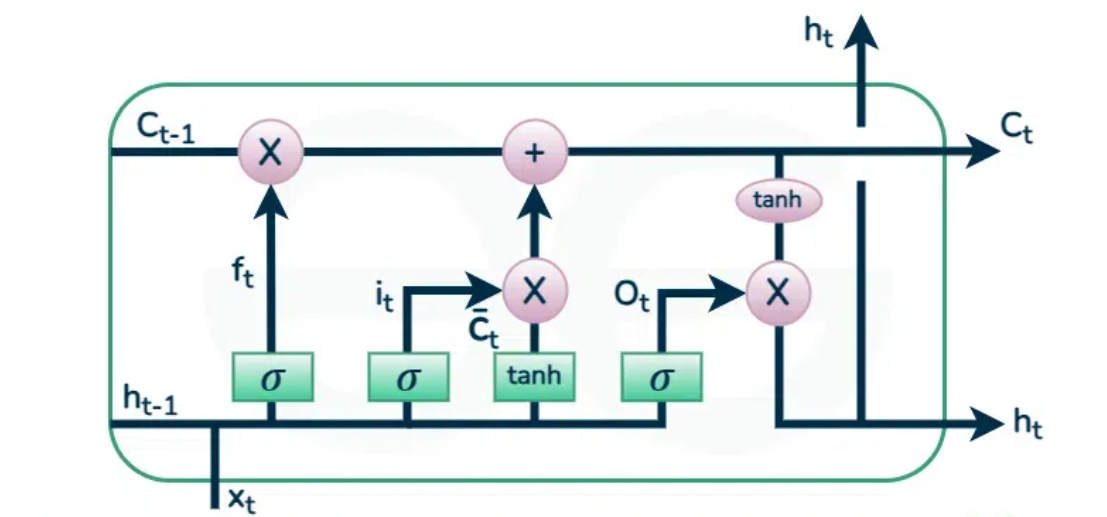
\includegraphics[width=0.9\linewidth]{Figures/LSTM.png}
	\caption{LSTM Architecture.}
	\label{/LSTM.png}
\end{figure}
Forget Gate: Decides what information to discard from the cell state
\[
f_t = \sigma \left( W_f \cdot [h_{t-1}, x_t] + b_f \right)
\]

Input Gate: Determines what new information to add to the cell state
\[
i_t = \sigma \left( W_i \cdot [h_{t-1}, x_t] + b_i \right)
\]
\[
\tilde{C}_t = \tanh \left( W_c \cdot [h_{t-1}, x_t] + b_c \right)
\]

Output Gate: Controls what information to output from the cell state
\[
o_t = \sigma \left( W_o \cdot [h_{t-1}, x_t] + b_o \right)
\]
\[
h_t = o_t \odot \tanh(C_t)
\]

It is worth mentioning that Bidirectional LSTM networks extend the traditional LSTM architecture by processing data in both forward and backward directions. This approach enables the network to capture dependencies from both past and future contexts, improving its ability to resolve temporal dependencies. Bidirectional LSTMs are particularly effective at handling multidimensional problems, encapsulating spatially and temporally distributed information, and dealing with incomplete data through flexible connection mechanisms \cite{hochreiter1997long}. 
\section{ Transformer Architecture}
The Transformer architecture is a deep learning model introduced in June 2017 by Vaswani et al. from Google Brain. Their paper, titled "Attention Is All You Need," presented a groundbreaking approach to processing sequential data through the use of a self-attention mechanism. This innovative method allows the model to assign different levels of importance to various parts of the input, enabling it to capture long-range dependencies much more effectively than earlier models like RNNs and LSTMs.The original Transformer model is structured as a stack of six layers, where the output of each layer i serves as the input to the subsequent layer i+1, continuing this process until the final prediction is reached.It features a six-layer encoder on the left and a corresponding six-layer decoder on the right,  both of which work together to transform input sequences into meaningful outputs. Each encoder and decoder consists of six identical layers that allow the model to process and generate language efficiently \cite{rothman2021transformers}.
\begin{figure}[htbp]
	
	\centerline{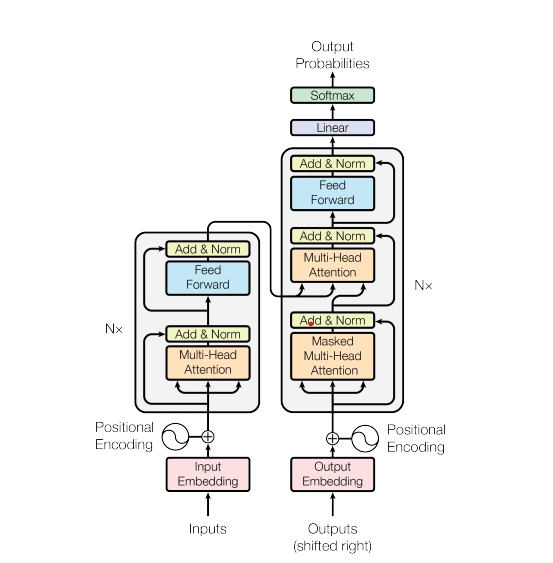
\includegraphics[width=.6\linewidth]{
			Figures/trasformers.png}}
	\caption{The Transformer - model architecture..}
	\label{trasformers.png}
	
\end{figure}
\subsection{Encoder and Decoder Stacks}
\textbf{Encoder:} Each layer in the encoder consists of two sub-layers: \\
Multi-head self-attention mechanism: This allows the model to focus on different parts of the input sequence. \\
Position-wise feed-forward network: A fully connected network applied to each position separately and identically. \\
Residual Connections: Residual connections are applied around each sub-layer, followed by layer normalization. The output of each sub-layer is computed as Layer Norm(x + Sublayer(x)). \\
Output Dimension: All sub-layers and embedding layers output vectors of dimension d-model = 512.\\
\textbf{Decoder:} Similar to the encoder, the decoder also has 6 identical layers, each containing the same two sub-layers:
Multi-head self-attention mechanism ,
Position-wise feed-forward network. \\
Additional Sub-layer: The decoder includes a third sub-layer that performs multi-head attention over the output of the encoder stack. \\
Residual Connections and Normalization: Like the encoder, residual connections are applied around each sub-layer, followed by layer normalization. \\
Masked Self-Attention: The self-attention mechanism in the decoder is modified to prevent positions from attending to subsequent positions, ensuring that predictions for position i depend only on the known outputs at positions before i \cite{vaswani2017attention}.
\begin{figure}[htbp]
	
	\centerline{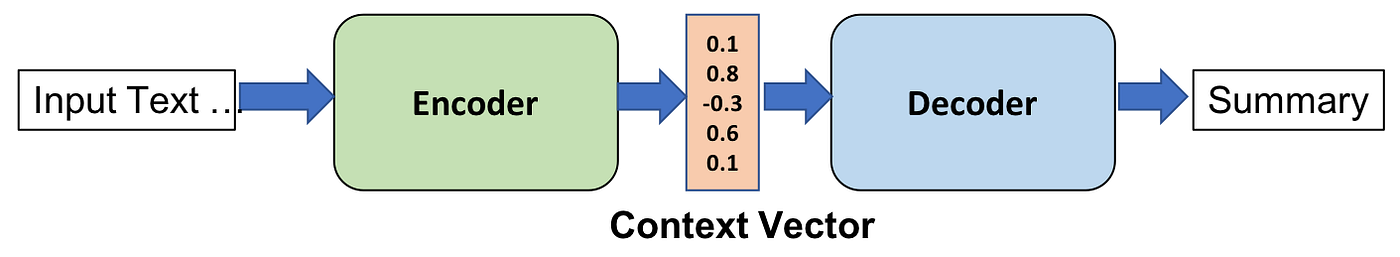
\includegraphics[width=.8\linewidth]{
			Figures/incoderDecoder.png}}
	\caption{Encoder and Decoder Stacks}
	\label{incoderDecoder.png}
	
\end{figure}
\subsection{Self-Attention Mechanism}
Self-attention is a mechanism that allows the model to weigh the importance of different words in a sequence relative to each other. This is crucial for understanding context and relationships between words \cite{vaswani2017attention}.
\subsection{Query, Key, and Value Vectors:}
\textbf{Query Vectors (Q):} Generated from the input word's embedding and represent the word's role in finding relevant information in other words.\\
\textbf{Key Vectors (K):} Derived similarly from embedding and serve as a comparison standard for each word.\\
\textbf{Value Vectors (V):} Contain the actual information to be passed on and are weighted according to relevance determined by the Query and Key comparison \cite{vaswani2017attention}.. 
\subsection{Self-Attention Calculation:}
The score is computed by taking the dot product of the Query vector of a word with the Key vectors of all other words. This score determines how much focus should be placed on each word when encoding the current word.
The scores are scaled and passed through a softmax function, producing a distribution of attention weights. \\
Each Value vector is weighted by these attention scores and summed to produce the final output of the self-attention layer\cite{vaswani2017attention}.
\subsection{Role of Multi-Head Attention}
Multi-head attention enhances the model’s ability to focus on different aspects of the input by creating multiple sets of Query, Key, and Value vectors. Each set is processed independently and then combined. \\
This approach allows the model to attend to information from different representation subspaces at different positions, improving its ability to capture complex relationships\cite{vaswani2017attention}.
\subsection{Positional Encoding:}
Since self-attention mechanisms do not inherently capture the order of words, positional encoding is added to the word embeddings to provide information about the relative position of each word in the sequence.
These encodings are added directly to the input embeddings, allowing the model to consider both the position and the content of 
each word during processing\cite{alammar2018illustratedtransformer}.
\subsection{Transformers in NLP}
Transformers have revolutionized the field of Natural Language Processing (NLP) by introducing a powerful and efficient way to handle textual data. This advancement has led to the creation of highly effective models like BERT and GPT, with its deep bidirectional context, excels at understanding and improving performance across various NLP tasks. GPT, on the other hand, is renowned for generating coherent and contextually relevant text, significantly advancing applications such as text generation and translation\cite{devlin2019bert}.\\
\textbf{Scalability:} Transformers efficiently handle large datasets and long sequences, overcoming the limitations of RNNs. This scalability allows for training with billions of parameters, enhancing model capabilities.\\
\textbf{Rich Contextual Understanding: }The self-attention mechanism in transformers captures relationships between words across the entire sequence, enabling deep contextual understanding and more accurate language processing.\\
\textbf{Model Efficiency:} Transformers enable parallel processing, which speeds up training and makes them more efficient than sequential models like RNNs. This efficiency supports the rapid development and deployment of advanced language models\cite{vaswani2017attention}.
\section{ Emergence of Large Language Models (LLMs)}

Large Language Models (LLMs) are advanced artificial intelligence systems designed to process and generate human-like text. They are typically based on transformer architectures and are characterized by their enormous scale, with billions of parameters. LLMs are pre-trained on vast amounts of text data in a self-supervised manner, enabling them to develop a broad understanding of language. They are capable of performing a wide range of tasks with minimal task-specific fine-tuning, often achieving significant performance improvements through few-shot or zero-shot learning\cite{brown2020language}.
\subsection{Scaling in Large Language Models (LLMs)}
Scaling is crucial in the evolution of large language models. The history of scaling shows that increasing both model size and dataset size leads to significant improvements in performance across various NLP tasks. For instance, early work by Brants et al. (2007) demonstrated the benefits of using language models trained on vast datasets, such as 2 trillion tokens, which led to significant advancements in machine translation quality. This was followed by efforts like those of Heafield et al. (2013), who scaled traditional models to Web-scale data, and Jozefowicz et al. (2016), who scaled LSTMs to 1 billion parameters, achieving state-of-the-art results on large benchmarks.The advent of transformer-based models marked a significant shift.Models like BERT, GPT-2, and GPT-3, with their enormous parameter counts—up to 175 billion for GPT-3—demonstrated that scaling up not only the model but also the dataset size yields substantial gains in performance. Researchers like Kaplan et al. (2020) and Hoffmann et al. (2022) studied how scaling affects model performance, proposing power laws that show a predictable relationship between model size, dataset size, and performance. These studies emphasized the importance of scaling for the continued progress of LLMs\cite{touvron2023llama}.
\subsection{Pre-training}
Pre-training is a crucial stage in developing Large Language Models (LLMs), where the model learns from extensive unlabeled datasets through a process called self-supervision. This stage allows the model to recognize and internalize a wide range of linguistic patterns, laying the groundwork for fine-tuning on specific tasks.\\
Several pre-training objectives have been implemented to maximize the effectiveness of this learning process, each offering distinct benefits to the model's performance
\textbf{Full Language Modeling:} Used since GPT-2, this approach trains decoder-only models to predict the next token in a sequence based on previous tokens. This autoregressive method enables models like GPT-3 to generate coherent and contextually relevant text.\\
\textbf{Prefix Language Modeling: }Employed in encoder-decoder and non-causal decoder-only models, this technique uses a non-causal (considering both past and future tokens) prefix for predicting subsequent tokens, offering more flexibility and enhancing the model's adaptability across various language tasks.\\
\textbf{Masked Language Modeling: }Popularized by BERT, this method involves masking certain tokens in the input text and training the model to predict them, helping the model understand word context. An extension, span corruption, masks entire text spans for prediction, further improving contextual comprehension\cite{wang2023language}.
\begin{figure}[htbp]
	
	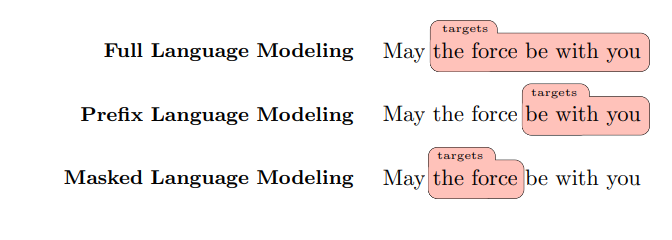
\includegraphics[width=1\linewidth]{Figures/pretraining.png}
	\caption{Training Tokenization in Full, Prefix, and Masked Language Modeling.}
\end{figure}
\subsection{Fine-tuning }
Fine-tuning has been the most common approach for adapting LLMs to specific tasks. After pre-training on large datasets, these models are further trained on smaller, supervised datasets tailored to the desired task. Fine-tuning updates the weights of the pre-trained model, allowing it to excel at specific tasks like sentiment analysis, machine translation, or question answering. The main advantage of fine-tuning is that it often results in strong performance on task-specific benchmarks. However, it comes with challenges, such as the need for a new large dataset for every task, the risk of overfitting to narrow distributions, and potential poor generalization to out-of-distribution examples\cite{touvron2023llama}.
\subsection{Few-Shot, One-Shot, and Zero-Shot Learning}
Few-shot, one-shot, and zero-shot learning represent different paradigms of using LLMs without extensive fine-tuning. These methods involve using pre-trained models to perform tasks with minimal task-specific data.\\
\textbf{Few-Shot Learning} involves giving the model a few examples (typically 10-100) of the task during inference. This approach reduces the need for large, task-specific datasets and limits the risk of overfitting to narrow data distributions. However, few-shot results are generally not as strong as those from fully fine-tuned models.\\
\textbf{One-Shot Learning} is similar to few-shot learning but uses only a single example alongside a natural language description of the task. This method mirrors how humans are often instructed for tasks, making it an interesting approach for tasks where providing multiple examples is impractical.\\
\textbf{Zero-Shot Learning} requires the model to perform a task based solely on a natural language description, with no examples provided. While this method offers maximum flexibility and robustness, it is also the most challenging for models. Zero-shot performance is often weaker than few-shot or one-shot, but it represents a significant step towards task-agnostic AI, where models can generalize across a wide range of tasks with minimal human intervention\cite{brown2020language}.
\subsection{Evaluation Datasets and Tasks}
Evaluating Large Language Models (LLMs) is essential for determining their effectiveness and limitations in comprehending and generating human language. This evaluation typically falls into two primary categories:
\begin{itemize}
	\item Natural Language Understanding (NLU):This measures the model's proficiency in comprehending language, encompassing tasks such as sentiment analysis, text classification, natural language inference (NLI), question answering (QA), commonsense reasoning (CR), mathematical reasoning (MR), and reading comprehension (RC).
	\item Natural Language Generation (NLG):This assesses the model's capability to produce text based on given context. It includes tasks like summarization, sentence completion, machine translation (MT), and dialogue generation.
\end{itemize}
\textbf{Benchmarks} play a critical role in evaluating LLMs, providing standardized tests to measure their performance across various tasks:
\begin{itemize}
	\item MMLU: Measures model knowledge from pretraining and evaluates performance in zero-shot and few-shot scenarios across 57 subjects, testing world knowledge and problem-solving abilities.
	\item SuperGLUE: An advanced benchmark that builds on GLUE, assessing tasks like question answering and natural language inference. It is designed to test deeper aspects of language understanding and requires significant advancements in various learning methodologies.
	\item BIG-bench: A large-scale benchmark for evaluating LLMs across diverse tasks including reasoning, creativity, ethics, and domain-specific knowledge.
	\item GLUE: A foundational benchmark for evaluating and analyzing natural language understanding, offering a range of resources for model assessment\cite{Naveed2024}.
\end{itemize}
\section{Popular Models and Datasets}
Large Language Models (LLMs) like GPT-3, GPT-4, and BERT have revolutionized NLP by leveraging vast datasets such as Common Crawl and WebText. These datasets provide a diverse linguistic foundation, enabling models to perform a wide range of tasks with remarkable accuracy and contextual understanding.
\subsection{GPT-N Models}
GPT models are advanced autoregressive language models that generate substantial and complex machine-produced text from minimal input. They leverage deep learning techniques to mimic human text generation by predicting the current value based on preceding values.
NLP models initially struggled with tasks outside their training sets due to data restrictions. OpenAI addressed this with GPT-1,introduced in 2018.
\begin{itemize}
	\item GPT-1, trained on the BooksCorpus dataset, utilized a 12-layer transformer decoder with self-attention. Its pre-training allowed for zero-shot performance on various tasks, demonstrating the potential of generative language models.
	\item In 2019, GPT-2 improved upon GPT-1 by using a larger dataset and 1.5 billion parameters (compared to GPT-1’s 117 million). It excelled in tasks like translation and summarization, enhancing accuracy in recognizing long-distance relationships.
	\item GPT-3, released later, featured around 175 billion parameters and was trained on the Common Crawl dataset. It could generate human-like text, perform basic math, and write code. Despite its capabilities, its size and cost made it challenging to implement.
	\item GPT-4, launched in March 2023, advanced further with multimodal capabilities and context windows of up to 32,768 tokens. It incorporates reinforcement learning for better alignment with human input and policy\cite{yenduri2023gpt}
\end{itemize}
\subsection{BERT}
BERT (Bidirectional Encoder Representations from Transformers) is a groundbreaking language representation model that pretrains deep bidirectional representations from unlabeled text by jointly conditioning on both left and right contexts in all layers. This bidirectional approach enables BERT to be fine-tuned with just a single additional output layer for various tasks, such as question answering and language inference, without the need for extensive architectural modifications. BERT has achieved remarkable performance, setting new state-of-the-art results across eleven NLP tasks, including a GLUE score of 80.5\%, MultiNLI accuracy of 86.7\%, SQuAD v1.1 F1 score of 93.2\%, and SQuAD v2.0 F1 score of 83.1\%. Its combination of conceptual simplicity and empirical effectiveness makes BERT a powerful and versatile tool for a wide range of natural language processing applications\cite{devlin2019bert}.
\subsection{T5}
The T5 (Text-To-Text Transfer Transformer) model represents a unified framework for natural language processing (NLP), designed to address various text processing tasks by treating them as "text-to-text" problems. This approach involves converting all tasks into a format where both input and output are text, allowing the same model, objective, and training procedure to be applied across different tasks. T5 leverages extensive pre-training on a large, unlabeled dataset, enabling it to develop general-purpose knowledge that enhances its performance on a range of NLP tasks, such as question answering, document summarization, and sentiment classification\cite{raffel2023exploring}.
\subsection{LLAMA2}
\subsection{WebText }
WebText is a dataset developed by OpenAI to encapsulate a wide variety of high-quality web content. It comprises text sourced from outbound links on popular websites like Reddit, chosen based on their popularity and the quality of their content. Unlike Common Crawl, which indiscriminately includes a broad range of web pages, WebText is more selective, focusing on high-quality, engaging material. Although smaller in size compared to Common Crawl, WebText is curated to ensure the text reflects diverse, well-written content, making it particularly valuable for training language models to produce coherent and contextually appropriate text\cite{radford2019language}.
\subsection{RuleTaker}
RuleTaker is a collection of datasets designed to assess the deductive reasoning capabilities of language models. Each dataset includes a set of facts, rules, and a boolean question that the model must use logical reasoning to answer. The datasets feature synthetic subsets requiring various levels of reasoning complexity, with different numbers of deduction steps necessary to reach an answer. Among the datasets are the Bird dataset, which illustrates McCarthy’s abnormality problem , the Electricity dataset, which models appliance functions, and the ParaRules corpus, where sentences like “Bob is cold” are paraphrased to “In the snow sits Bob, crying from being cold.” The collection comprises 580,000 training examples, 84,000 validation examples, and 173,000 testing examples\cite{helwe2024}.
\begin{figure}
	\centering
	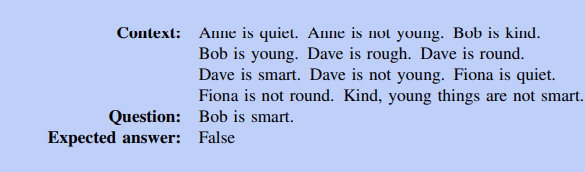
\includegraphics[width=0.7\linewidth]{Figures/dataset-exmple.png}
	\caption{exammple of RuleTaker dataset }
\end{figure}
\section{Challenges and Limitations}
LLMs have greatly advanced NLP, but they also present challenges such as high computational costs, issues with adversarial robustness, and difficulties in interpretability. As these models scale, they encounter new challenges in scalability, privacy, and real-time processing. Ongoing research is exploring multi-modality, transfer learning, and continuous learning, which bring additional complexities and highlight the evolving impact of LLMs in practical applications\cite{Naveed2024}.
\subsection{ Computational Cost}
Training large language models (LLMs) demands significant computational resources, leading to higher production costs and environmental concerns due to the substantial energy used in large-scale training. Although enhancing computational resources can boost performance, the gains diminish over time when the size of the model and dataset stay constant, adhering to the power law of diminishing returns.
\subsection{Overfitting}
Despite their advanced learning abilities, they can overfit to noisy or unusual patterns in their large training datasets, which may result in generating nonsensical responses. The ongoing discussion about Memorization versus Generalization in LLMs revolves around finding an optimal balance. Memorization helps the model retain specific details from its training, allowing it to answer precise questions accurately. On the other hand, generalization enables the model to make predictions and generate responses for new, unseen inputs, which is crucial for handling diverse real-world tasks. The challenge is to find the right balance: excessive memorization can lead to overfitting, reducing the model's flexibility and ability to handle novel inputs.
\subsection{ Interpretability and Explainability}
The "black-box" nature of LLMs makes it difficult to understand how they make decisions, which is vital for gaining broader acceptance and trust, particularly in sensitive areas. Although these models have advanced capabilities, the lack of transparency into their workings limits their effectiveness and reliability. Efforts are underway to enhance the explainability of LLMs to build user trust and promote responsible use of AI. Understanding how LLMs generate their responses is crucial for ensuring they align with human values and legal standards.
\subsection{ Hallucinations}
LLMs sometimes produce "hallucinations," or responses that, despite appearing plausible, are incorrect or do not match the provided information. These hallucinations can be classified into three types:

\begin{itemize}
	\item Input-conflicting hallucination: When the model generates responses that do not align with the user's input.
	\item Context-conflicting hallucination: When the model produces content that contradicts information it has previously generated.
	\item Fact-conflicting hallucination: When the model creates responses that conflict with established knowledge.
\end{itemize}
\subsection{Privacy Concerns}
As Large Language Models (LLMs) have become more complex and sizable, privacy concerns have intensified, particularly regarding data sharing and potential misuse. Risks include the creation of harmful content, evasion of filters, and issues related to data privacy, especially in areas like e-commerce where safeguarding customer information is vital. When LLMs are trained on private data and then made publicly available, additional privacy risks arise. Since LLMs can memorize phrases from their training data, there's a danger that these phrases could be exploited by malicious actors to retrieve sensitive information, thus threatening personal privacy.
\subsection{Real-Time Processing}
Real-time processing in Large Language Models (LLMs) is crucial for many applications, particularly as mobile AI solutions become more popular and concerns about information security and privacy grow. However, LLMs typically consist of hundreds of layers and millions of parameters, which create significant challenges for real-time processing due to their high computational demands and the limited storage capacity of hardware platforms, especially in edge computing environments. Although efforts such as MobileBERT attempt to lessen memory usage, they still encounter considerable execution overhead because of the extensive number of model layers, resulting in high inference latency.
\section{Domains of Application}
The use of Large Language Models (LLMs) in various downstream tasks has become increasingly prevalent in both AI research and industry, with new applications being identified and explored regularly. These models, which excel at understanding and generating human-like text, are finding valuable applications across diverse fields. 
\subsection{Law} 
In the legal field, Large Language Models (LLMs) can support the analysis of legal documents by assisting with tasks such as generating initial coding for datasets, identifying key themes, and classifying information accordingly. This synergy between legal professionals and LLMs has been effective in examining legal texts, such as court opinions on theft, enhancing both the efficiency and quality of legal research. Additionally, LLMs have been tested for their capability to generate explanations of legal terms, with a focus on improving factual accuracy by integrating sentences from relevant case law. By incorporating pertinent case law, these enhanced models can produce more accurate and relevant explanations with fewer factual errors. Furthermore, LLMs can be specialized with domain-specific knowledge to tackle legal reasoning tasks and address legal queries effectively \cite{Naveed2024}.
\subsection{Cybersecurity}
large Language Models (LLMs) have garnered significant attention in the field of cybersecurity. Recent research has highlighted their potential in addressing software bugs created by human developers and identifying cybersecurity threats. For example, Arora et al. have proposed methods for utilizing LLMs to evaluate cyber threats on social media through sentiment analysis. LLMs are also employed to detect cybersecurity-related information in Open Source Intelligence (OSINT), aiding in the identification of potential cyber threats. Additionally, LLMs have shown promise in detecting scams, such as phishing. Initial tests with models like GPT-3.5 and GPT-4 have demonstrated their ability to recognize common phishing indicators in emails. While LLMs exhibit considerable potential in cybersecurity, improving their reasoning abilities could enhance their effectiveness further, such as in uncovering zero-day vulnerabilities in open-source software by analyzing logic and source code\cite{helwe2024}.
\subsection{Medicine}
The integration of Large Language Models (LLMs) into medicine is transforming both healthcare delivery and research. In clinical settings, LLMs are increasingly utilized in decision support systems to offer evidence-based treatment recommendations. By analyzing patient data and medical literature, these models can assist in diagnosing conditions, suggesting relevant tests, and proposing effective treatment options. Additionally, LLMs improve patient interactions through applications like chatbots that answer questions about symptoms and medications, schedule appointments, and provide health advice.\\
In medical research, LLMs help sift through vast amounts of literature to extract, filter, and summarize relevant information, identify key studies, and predict future research directions. They also play a role in medical education by generating training materials, creating exam questions, explaining complex topics, and offering personalized feedback. Furthermore, LLMs simulate patient interactions, aiding students in honing their clinical skills \cite{Naveed2024}.

\subsection{journalism}
Large Language Models (LLMs) offer valuable support to journalists, especially in fact-checking and news verification. They can process and cross-reference large volumes of data with established knowledge bases. Research has demonstrated that LLMs, such as GPT-3.5, can be used to detect fake news by providing rationales that enhance other models like BERT, which can then be fine-tuned for this purpose .
In addition to fact-checking, LLMs are useful for analyzing political debates, helping journalists to identify key themes, monitor how discussions evolve, and evaluate sentiments. They can also assist in detecting logical fallacies and underlying motives in political discourse and propaganda . By enhancing their reasoning capabilities, LLMs can uncover deeper insights into propaganda and misinformation, making them a powerful tool for modern journalism\cite{helwe2024}.

\section{Conclusion}
This chapter has outlined the evolution and significance of Natural Language Processing (NLP), from early neural networks to advanced Large Language Models (LLMs). We covered key concepts in neural networks and the transformative impact of the Transformer architecture. The exploration of LLMs highlighted their emergence, scaling, and the intricacies of pre-training and fine-tuning. We also discussed various challenges, including computational costs, interpretability, and privacy concerns. Finally, the chapter reviewed the applications of LLMs in fields like law, cybersecurity, medicine, and journalism, showcasing their potential and the ongoing need for further development.